\documentclass[11pt,a4paper]{article}
\usepackage[T1]{fontenc}
\usepackage[utf8]{inputenc}
\usepackage{lmodern}
\usepackage{microtype}
\usepackage[a4paper,margin=25mm,headheight=14pt]{geometry}
\setlength{\emergencystretch}{2em}
\usepackage[numbers,sort&compress]{natbib}
\usepackage{amsmath,amssymb,amsthm}
\usepackage{booktabs}
\usepackage{multirow}
\usepackage{graphicx}
\usepackage[font=small,labelfont=bf]{caption}
\usepackage{enumitem}
\usepackage{xcolor}
\usepackage{tikz}
\usetikzlibrary{positioning,arrows.meta,fit}
\usepackage{fancyhdr}
\usepackage{lastpage}
\usepackage{hyperref}
\usepackage[nameinlink,noabbrev]{cleveref}
\hypersetup{colorlinks=true,linkcolor={blue!50!black},citecolor={blue!50!black},urlcolor={blue!50!black}}
\captionsetup[figure]{name=Fig.}
\setlist{nosep}
\graphicspath{{../results/figures/}}
\pagestyle{fancy}
\fancyhf{}
\lhead{\small Supplier selection, ordering and transport planning}
\rhead{\small Page \thepage\ of \pageref*{LastPage}}
\renewcommand{\headrulewidth}{0.4pt}
\newcommand{\E}{\mathbb{E}}
\newcommand{\Var}{\operatorname{Var}}

\begin{document}

%% ================================================================== Summary
\thispagestyle{empty}
\begin{center}
{\LARGE\bfseries Supplier Selection, Ordering and Transport Planning\\[3pt] under Uncertain Deliveries\par}
\vspace{6pt}
{\normalsize Xiangyu Luo\par}
{\small CUMCM 2021 Problem C; undergraduate mathematical modelling training, Southwest Petroleum University (2023)\par}
\vspace{10pt}
{\Large\bfseries Summary\par}
\end{center}

A manufacturer turns three raw materials into 28{,}200\,m$^3$ of product per week, buys them from 402 suppliers whose deliveries deviate from their orders, ships them with eight carriers that lose part of every load, and must always hold two weeks of production in stock.
Five years of weekly records show that the firm received less than it needed in 173 of 240 weeks although it ordered a third more, so the central question behind all four problems is how much a supplier can actually be relied on for.
We answer it with a supply model that separates two quantities: the \emph{sustained capacity} of a supplier, the largest quantity it delivered in every week of some four-week run, and the empirical distribution of its delivered-to-ordered ratio.
Every plan is then judged by the probability that the stock stays above two weeks of demand in all 24 planning weeks, estimated on simulated scenarios that were not used to build the plan.

For Problem 1 we derive the importance of a supplier from its contribution to the stock balance, which is the product it can be expected to supply per week, $K_i\bar\rho_i/\alpha_i$.
The 50 highest-ranked suppliers hold 98.8\% of the total sustained capacity.
An independent entropy-weight TOPSIS evaluation on five indicators selects 42 of the same 50, and the ranking changes by at most two suppliers when the capacity definition or the reliability measure is changed (Kendall's $\tau$ 0.62--0.99).

For Problem 2 we formulate the selection of the fewest suppliers as a chance-constrained 0--1 programme and solve its sample average approximation exactly.
Eighteen suppliers keep the two-week stock in every week with an out-of-sample probability of 96.7\% when they are ordered at capacity, whereas the fifteen suppliers suggested by expected values achieve only 40\%; repeated approximations with 100 to 400 scenarios return 17 or 18 suppliers with at least 15 in common with our choice.
A linear programme whose safety stock grows with the accumulated delivery uncertainty yields the cheapest order plan, at the historical cost per unit of product and with 91.6\% compliance, and a carrier-assignment programme lowers the expected transport loss to 0.58\%, against 1.38\% for random feasible assignments.

For Problem 3 we show that per unit of product A, B and C cost almost the same, so that preferring A and avoiding C is equivalent to minimising raw volume.
The volume-minimal plan buys all available A, cuts the volume of C by 61\% and the total volume by 4.0\%, and costs only 0.2\% more.

For Problem 4 we bisect on the weekly production for which a plan over all suppliers still meets the stock requirement with 95\% probability and obtain about 37{,}700\,m$^3$ per week, 34\% above the current level, with the carriers far from saturation.
Stress tests with correlated deliveries, alternative ratio caps and demand changes confirm the selection of Problem 2, whereas the production limit of Problem 4 ranges from $-11\%$ to $+101\%$ across capacity definitions and should be read together with the definition it rests on.

\medskip
\noindent\textbf{Keywords:} supplier selection; chance-constrained programming; sample average approximation; safety stock; carrier assignment; out-of-sample validation

\newpage
\begingroup
\small
\setlength{\parskip}{0pt}
\tableofcontents
\endgroup
\newpage

%% ================================================================== 1
\section{Introduction}

\subsection{Problem Background}
A manufacturer that depends on many small and unreliable suppliers faces two risks at once.
If it relies on too few of them, a single short delivery can interrupt production; if it spreads its orders over too many, it pays for administration, transport and quality control of a large and fragmented supply base.
Classical supplier-selection models balance these risks with deterministic capacities and multi-criteria scores \citep{aissaoui2007,ho2010}, but in practice the quantity a supplier delivers is itself random, and a plan that is feasible on average may fail in most realisations.

The firm in this problem makes one product from three interchangeable raw materials, A, B and C.
One cubic metre of product needs 0.60\,m$^3$ of A, 0.66\,m$^3$ of B or 0.72\,m$^3$ of C.
A and B cost 20\% and 10\% more per cubic metre than C, while transport and storage cost the same per cubic metre for all three materials.
The firm buys from 402 suppliers, each of which supplies only one material and delivers more or less than it was ordered.
Eight carriers move the material to the plant; each ships at most 6{,}000\,m$^3$ per week, loses a random fraction of what it ships, and the material of one supplier should be shipped by a single carrier whenever possible.
The firm produces 28{,}200\,m$^3$ of product per week, plans 24 weeks ahead and must at all times hold at least two weeks of production in raw-material stock.

\subsection{Restatement of the Problem}
The data consist of the weekly orders and deliveries of the 402 suppliers over 240 weeks (attachment~1) and the weekly loss rates of the eight carriers over the same weeks (attachment~2).
On this basis the problem asks four questions.
\begin{enumerate}[label=(\arabic*),itemsep=2pt]
\item Quantify how important each supplier is for keeping production going, and identify the 50 most important suppliers.
\item Find the smallest set of suppliers that can sustain production, and give for it the cheapest order plan and the transport plan with the lowest loss for the next 24 weeks.
\item Give order and transport plans that buy as much A and as little C as possible, in order to reduce transport and storage costs, while keeping transport losses small.
\item Determine by how much the weekly production could be raised with the existing suppliers and carriers, and give the corresponding plans.
\end{enumerate}

\subsection{Related Work}
Supplier selection has been studied as a multi-criteria decision problem and as an optimisation problem.
Multi-criteria methods such as the analytic hierarchy process, TOPSIS and their entropy-weighted variants rank suppliers by aggregated indicators \citep{ho2010,hwang1981}; they are transparent but say nothing about how many suppliers are needed.
Optimisation models choose suppliers and order quantities jointly, usually with known capacities and yields \citep{aissaoui2007}.
When deliveries are random, the natural requirement is that a service condition holds with high probability, which leads to chance-constrained programming \citep{charnes1959}.
Chance constraints are rarely tractable in closed form, but their sample average approximation (SAA), which replaces the probability by a frequency over sampled scenarios and allows a fixed fraction of them to fail, is a mixed-integer programme whose solutions converge to those of the true problem as the sample grows \citep{luedtke2008,pagnoncelli2009}.
On the ordering side, safety stocks proportional to the standard deviation of supply or demand over the protection interval are the classical answer to random yields \citep{silver2016}.
Our approach combines these elements: it estimates the uncertainty directly from the delivery records, uses SAA for the discrete selection, a safety-stock linear programme for the continuous order quantities, and judges every decision on independent scenarios.

\subsection{Overview of Our Work}
The four problems share one obstacle that determines the whole approach.
The data record what a supplier delivered, but this depends on what it was ordered, so capacities are not observed directly; at the same time deliveries deviate randomly from orders, so any plan that is computed from averages may fail.
We therefore begin with a supply model (\cref{sec:model}) that defines a capacity the records support and treats the delivery ratio as a random variable resampled from each supplier's own history.
The supply model feeds four decision models, one per problem, as shown in \cref{fig:flow}.
Problem 1 turns the supply model into an importance score and checks it against an independent multi-criteria evaluation (\cref{sec:q1}).
Problem 2 selects suppliers by a chance-constrained programme, plans orders with a safety stock that reflects the accumulated uncertainty and assigns carriers by a mixed-integer programme (\cref{sec:q2}).
Problems 3 and 4 reuse the order and transport models with a different objective (\cref{sec:q3}) and a variable demand (\cref{sec:q4}).
Because every model relies on the same simulated stock dynamics, we can test all decisions in the same way, which we do in \cref{sec:sensitivity} for correlated deliveries, alternative capacity definitions and parameter changes.

\begin{figure}[ht]
\centering
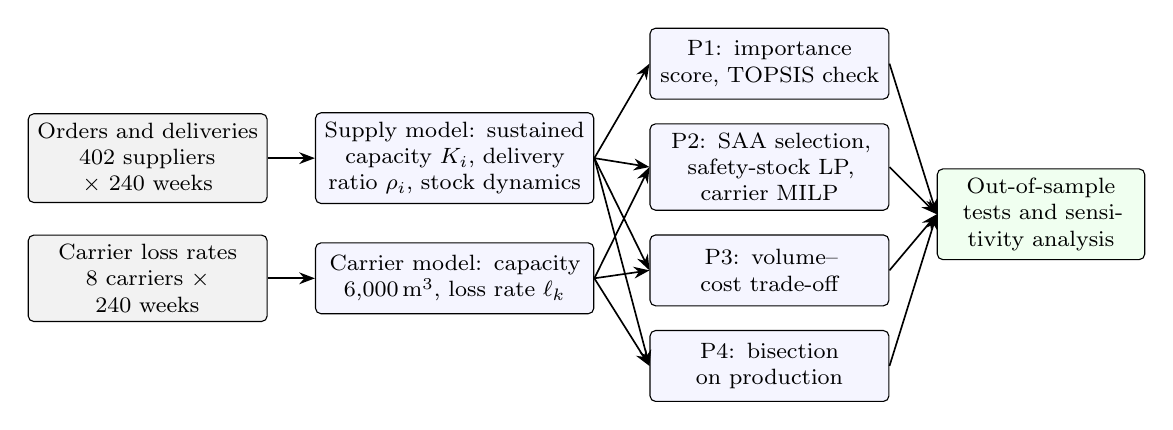
\begin{tikzpicture}[
  box/.style={draw, rounded corners=2pt, align=center, font=\footnotesize, minimum height=9mm, text width=28mm, fill=blue!4},
  dat/.style={box, fill=gray!10},
  arr/.style={-{Stealth[length=2mm]}, semithick}]
\node[dat] (d1) {Orders and deliveries\\402 suppliers $\times$ 240 weeks};
\node[dat, below=4mm of d1] (d2) {Carrier loss rates\\8 carriers $\times$ 240 weeks};
\node[box, right=6mm of d1, text width=33mm] (sm) {Supply model: sustained capacity $K_i$, delivery ratio $\rho_i$, stock dynamics};
\node[box, right=6mm of d2, text width=33mm] (tm) {Carrier model: capacity 6{,}000\,m$^3$, loss rate $\ell_k$};
\node[box, right=7mm of sm, yshift=12mm] (q1) {P1: importance score, TOPSIS check};
\node[box, below=3mm of q1] (q2) {P2: SAA selection, safety-stock LP, carrier MILP};
\node[box, below=3mm of q2] (q3) {P3: volume--cost trade-off};
\node[box, below=3mm of q3] (q4) {P4: bisection on production};
\node[box, right=6mm of q2, yshift=-6mm, text width=24mm, fill=green!6] (val) {Out-of-sample tests and sensitivity analysis};
\draw[arr] (d1) -- (sm);
\draw[arr] (d2) -- (tm);
\foreach \q in {q1,q2,q3,q4} \draw[arr] (sm.east) -- (\q.west);
\draw[arr] (tm.east) -- (q2.west);
\draw[arr] (tm.east) -- (q3.west);
\draw[arr] (tm.east) -- (q4.west);
\foreach \q in {q1,q2,q3,q4} \draw[arr] (\q.east) -- (val.west);
\end{tikzpicture}
\caption{Structure of the work: one supply model and one carrier model feed the four decision models, whose results are all tested on independent scenarios.}\label{fig:flow}
\end{figure}

%% ================================================================== 2
\section{Assumptions and Justifications}\label{sec:assumptions}

The models rest on five assumptions.
Each is stated together with the reason why we consider it acceptable and the place where its consequences are tested.
\begin{enumerate}[label=A\arabic*.,leftmargin=*,itemsep=4pt]
\item A supplier can deliver up to its sustained capacity $K_i$ in any week, but not reliably more. By its definition in \cref{eq:K}, a supplier with capacity $K_i$ delivered at least $K_i$ in every week of a whole month, which shows that the quantity is within its means; isolated spikes, which may come from clearing a backlog, are not treated as capacity. The length of the run is varied in \cref{sec:sens-window}.
\item The ratio of delivered to ordered quantity is random, independent across suppliers and weeks, and follows the supplier's historical distribution, including zero deliveries and with values capped at 1.5. The data contain no information about the causes of the deviations, and resampling the observed ratios preserves their actual spread and their heavy lower tail. Independence is tested against a block bootstrap of historical weeks in \cref{sec:sens-corr}, and the cap is varied in \cref{sec:sens-param}.
\item Orders up to the sustained capacity are delivered with the same ratio distribution as the historical orders. The records contain no orders of this size for some suppliers, and keeping the observed distribution is the least informative extrapolation.
\item Each carrier ships at most 6{,}000\,m$^3$ per week, and its loss rate in a planning week is random with the historical distribution; for planning we use its historical mean. The capacity is given in the problem statement, and the transport plans are afterwards replayed against the actual historical loss rates.
\item Material delivered in a week can be used for production in the same week, the stock at the beginning of the planning horizon equals two weeks of production, and the stock is measured in cubic metres of product equivalent. The problem gives no lead times, and the firm is already required to hold this stock; product equivalents make the three materials comparable.
\end{enumerate}

%% ================================================================== 3
\section{Notations}\label{sec:notation}

\begin{table}[ht]
\centering
\caption{Main symbols. Volumes are in m$^3$; prices are relative to the price of C.}\label{tab:notation}
\small
\begin{tabular}{lp{0.6\textwidth}}
\toprule
Symbol & Meaning \\
\midrule
$i$; $k$; $t$ & supplier ($1,\dots,402$); carrier ($1,\dots,8$); planning week ($1,\dots,24$) \\
$o_{i,w}$, $s_{i,w}$ & historical order and delivery of supplier $i$ in week $w=1,\dots,240$ \\
$K_i$, $W$ & sustained capacity of supplier $i$ (m$^3$/week); window length (weeks) \\
$\rho_{it}$; $\bar\rho_i$, $v_i$ & delivery ratio of supplier $i$ in week $t$; its mean and variance \\
$\alpha_i\in\{0.60,0.66,0.72\}$ & raw material per m$^3$ of product (A, B, C) \\
$p_i\in\{1.2,1.1,1.0\}$ & price per m$^3$ of supplier $i$'s material \\
$D$ & weekly production (28{,}200\,m$^3$ of product) \\
$x_{it}$ & order placed with supplier $i$ for week $t$ \\
$I_t$ & stock at the end of week $t$, in product equivalent \\
$y_i$; $z_s$ & 1 if supplier $i$ is selected; 1 if scenario $s$ may fail \\
$N$, $\varepsilon$ & number of SAA scenarios; allowed failure probability \\
$\sigma_t(x)$; $z$ & standard deviation of cumulative supply up to week $t$; safety factor \\
$f_{ik}$, $u_{ik}$, $\ell_k$ & volume of $i$ shipped by $k$; 1 if the pair is used; mean loss rate of $k$ \\
$\pi$ & compliance: probability that $I_t\ge 2D$ in all 24 weeks \\
\bottomrule
\end{tabular}
\end{table}

%% ================================================================== 4
\section{Data Description and Supply Model}\label{sec:model}

\subsection{Overview of the Records}
The 402 suppliers comprise 146 suppliers of A, 134 of B and 122 of C.
Every supplier received orders in some weeks, but in a typical week only a minority of them is active: the median supplier was ordered in about 69 of the 240 weeks.
Converted to product equivalents by dividing each quantity by $\alpha_i$, the firm ordered on average 37{,}124\,m$^3$ per week but received only 27{,}933\,m$^3$, and the deliveries fell short of the weekly demand in 173 weeks (\cref{fig:hist}).
The shortfall is therefore not caused by a lack of orders, but by deliveries that systematically fall behind them.
Of the delivered product, 36\% came from A, 34\% from B and 30\% from C, so the firm has historically used the three materials in similar proportions.

\begin{figure}[ht]
\centering
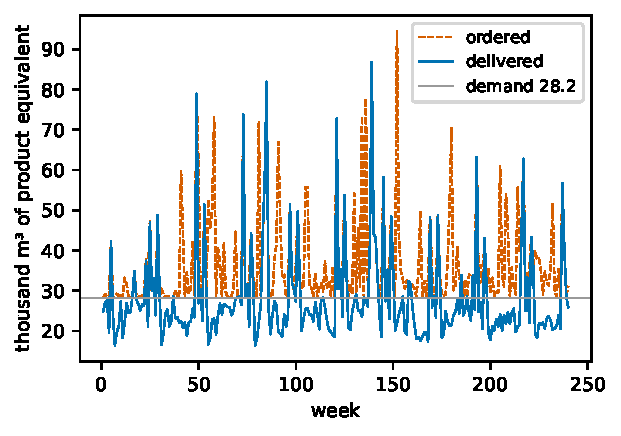
\includegraphics[width=0.62\textwidth]{history}
\caption{Weekly orders and deliveries of all 402 suppliers in product equivalent over the 240 recorded weeks, compared with the demand of 28{,}200\,m$^3$.}\label{fig:hist}
\end{figure}

Two features of the supplier records shape the supply model.
The first is that deliveries follow orders: for the 20 suppliers with the largest total deliveries, the logarithms of weekly orders and deliveries have a median correlation of 0.95.
A supplier that delivered little was mostly ordered little, so the historical deliveries are a lower bound on what a supplier can do rather than a measure of it.
The second feature is that deliveries deviate strongly from orders.
In 64\% of the supplier-weeks with an order the order was filled completely, but in 28\% nothing was delivered at all, mostly at small suppliers, and a few suppliers show isolated deliveries far above their usual level: the largest delivery of S151 is 21{,}267\,m$^3$, 34 times its median positive delivery, and that of S140 more than 3{,}000 times its median.
A model of supply must therefore distinguish a sustainable level from occasional spikes, and it must describe the deviation from orders as a random quantity.

\subsection{Sustained Capacity}
Because a single large delivery does not show that a supplier can deliver that much every week, we define capacity through persistence.
The sustained capacity of supplier $i$ is the largest quantity that it delivered in \emph{every} week of some run of $W$ consecutive weeks,
\begin{equation}\label{eq:K}
K_i = \max_{1\le w\le 241-W}\ \min\{s_{i,w}, s_{i,w+1},\dots,s_{i,w+W-1}\}.
\end{equation}
We take $W=4$, one month, as the base case.
The definition has three properties that make it suitable here.
It is never larger than the largest delivery and never smaller than the smallest, so it stays within the observed range; it ignores isolated spikes, because a spike would have to persist for $W$ weeks to count; and it decreases monotonically in $W$, so that $W$ acts as a single, interpretable dial between optimism and caution.
With $W=4$, S151 obtains a capacity of 779\,m$^3$ instead of its maximum of 21{,}267\,m$^3$, and S140 a capacity of 8\,m$^3$.
Only 225 suppliers have a positive sustained capacity; the others never delivered in four consecutive weeks.
Weighting each capacity by the mean delivery ratio and converting it to product, the total expected capacity is 81{,}778, 42{,}675, 31{,}156 and 28{,}011\,m$^3$ per week for $W=3,4,6,8$.
Short windows admit short bursts and suggest almost three times the demand, whereas with $W=8$ the capacity barely covers it, which already indicates that Problem 4 will depend on this choice (\cref{sec:sens-window}).

\subsection{Delivery Ratio}
For each supplier we collect the ratios $s_{i,w}/o_{i,w}$ over all weeks with a positive order, cap them at 1.5 and treat them as an empirical distribution from which the planning-week ratios $\rho_{it}$ are drawn independently (assumption A2).
The pooled distribution in \cref{fig:ratio} (left) is strongly bimodal.
Over all supplier-weeks with an order, 28\% of the ratios are zero, 36\% lie within 10\% of one and 8\% exceed the cap, the latter mostly for very small orders.
Large suppliers are much more reliable than small ones: the mean ratio of the 50 highest-ranked suppliers of \cref{sec:q1} lies between 0.54 and 1.23 and is close to one for most of them, whereas many small suppliers have zero-delivery probabilities above 50\%.
We keep each supplier's own distribution, rather than fitting a parametric family, because the probability mass at zero and the cap at 1.5 are both essential for the risk of falling below the stock requirement.

\begin{figure}[ht]
\centering
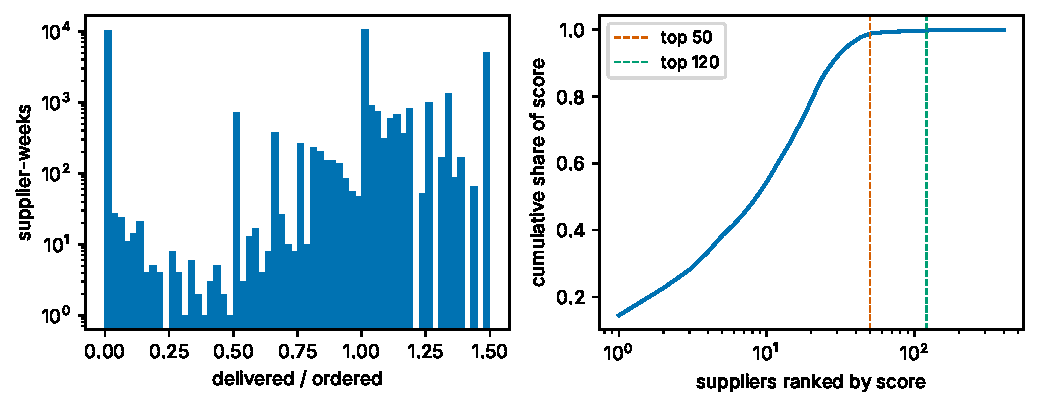
\includegraphics[width=0.95\textwidth]{data_ratio_pareto}
\caption{Left: distribution of the delivered-to-ordered ratio over all supplier-weeks with an order (logarithmic count axis, capped at 1.5). Right: cumulative share of the total importance score of \cref{sec:q1} held by the suppliers ranked by score.}\label{fig:ratio}
\end{figure}

\subsection{Stock Dynamics and Compliance}
In product equivalent the stock starts at $I_0=2D$ and evolves as
\begin{equation}\label{eq:stock}
I_t = I_{t-1} + \sum_i \frac{\rho_{it}x_{it}}{\alpha_i} - D,\qquad t=1,\dots,24,
\end{equation}
so that $I_t\ge 2D$ holds exactly when the cumulative supply keeps pace with the cumulative demand, $\sum_{\tau\le t}\sum_i\rho_{i\tau}x_{i\tau}/\alpha_i\ge tD$.
We call a plan \emph{compliant} in a scenario if this holds in all 24 weeks, and we denote by $\pi$ the probability of compliance, which we target at 95\%.
Requiring compliance in every week of the horizon is deliberately strict: a plan with $\pi=0.95$ keeps the full two-week buffer throughout the half year in 19 of 20 cases, and it almost never runs out of stock altogether.

Under assumption A2 the supply of a given plan has mean and variance
\begin{equation}\label{eq:moments}
\E\Big[\sum_{\tau\le t}\sum_i\frac{\rho_{i\tau}x_{i\tau}}{\alpha_i}\Big]=\sum_{\tau\le t}\sum_i\frac{\bar\rho_i x_{i\tau}}{\alpha_i},\qquad
\sigma_t(x)^2=\Var\Big[\sum_{\tau\le t}\sum_i\frac{\rho_{i\tau}x_{i\tau}}{\alpha_i}\Big]=\sum_{\tau\le t}\sum_i v_i\Big(\frac{x_{i\tau}}{\alpha_i}\Big)^2,
\end{equation}
where the variance is additive because the ratios are independent.
Two consequences guide the order model of \cref{sec:q2}.
The variance of the cumulative supply grows with $t$, so a plan needs more protection late in the horizon than early; and it grows with the square of each supplier's share, so concentrating orders on few suppliers is riskier than the expected values suggest.
Since the ratio distributions are far from normal, we use \cref{eq:moments} only to shape the safety stock and always measure $\pi$ by simulation.

\subsection{Carrier Loss Rates}\label{sec:carriers}
The eight carriers differ considerably in their losses (\cref{tab:carriers}).
A recorded loss of zero means that the carrier shipped nothing in that week, so we compute statistics over the active weeks only.
T3 loses on average 0.19\% of what it ships and T6 0.54\%, whereas T5 loses 2.89\%, fifteen times as much.
The distributions are skewed: most weeks have small losses, but several carriers occasionally reach the recorded maximum of 5\%, which is why the standard deviation of T6 exceeds its mean.
For a single week a carrier can therefore turn out worse than its average, but over a half-year plan the means decide the total loss, and their differences are large enough to make the choice of carrier worth optimising.

\begin{table}[ht]
\centering
\caption{Weekly loss rates of the carriers over the weeks in which they were active (in \%).}\label{tab:carriers}
\small
\begin{tabular}{lrrrr}
\toprule
carrier & active weeks & mean & standard deviation & 95th percentile \\
\midrule
T3 & 117 & 0.19 & 0.48 & 0.53 \\
T6 & 216 & 0.54 & 1.35 & 4.85 \\
T2 & 240 & 0.92 & 0.48 & 1.60 \\
T8 & 203 & 1.01 & 1.11 & 5.00 \\
T4 & 102 & 1.57 & 1.93 & 5.00 \\
T1 & 240 & 1.90 & 0.66 & 2.98 \\
T7 & 240 & 2.08 & 1.43 & 5.00 \\
T5 & 83 & 2.89 & 1.96 & 5.00 \\
\bottomrule
\end{tabular}
\end{table}

%% ================================================================== 5
\section{Model I: Supplier Importance (Problem 1)}\label{sec:q1}

\subsection{Analysis}
A supplier is important for production to the extent that it helps to keep the stock above the requirement.
In the stock balance \cref{eq:stock}, supplier $i$ contributes $\rho_{it}x_{it}/\alpha_i$ per week, and the largest order it can be relied on for is $K_i$.
Its expected contribution to production is therefore
\begin{equation}\label{eq:score}
Q_i = \frac{K_i\,\bar\rho_i}{\alpha_i}\quad\text{(m$^3$ of product per week)},
\end{equation}
which combines the three aspects that a reasonable notion of importance should contain: the scale of the supplier, through $K_i$; its reliability, through $\bar\rho_i$; and the value of its material for production, through $1/\alpha_i$.
Unlike indicators based on historical totals, $Q_i$ does not reward a supplier that delivered a lot only because it was ordered a lot, and it does not reward isolated spikes.
We rank all suppliers by $Q_i$ and, because a score always depends on modelling choices, we test the ranking in two ways: against an independent multi-criteria evaluation that does not use the supply model, and against variants of the score itself.

\subsection{Ranking and Concentration}
The ranking is extremely concentrated (\cref{fig:ratio}, right).
The largest supplier, S374, accounts for 14.5\% of the total score, the ten largest for 54\%, the twenty largest for 79\% and the fifty largest for 98.8\%; only 43 suppliers have a score above 100\,m$^3$ per week.
The 50 most important suppliers are listed in \cref{tab:top50}.
They include 19 suppliers of A, 11 of B and 20 of C, and they delivered 87.0\% of all historical supply.
The gap between 98.8\% of capacity and 87.0\% of history reflects the many small suppliers that delivered occasionally without ever sustaining a monthly level.
The concentration has a practical meaning for the following problems: since a handful of suppliers carries most of the capacity, the minimum supplier set of Problem 2 will be small, and its reliability will be governed by the delivery behaviour of these few suppliers.

\begin{table}[ht]
\centering
\caption{The 50 most important suppliers ranked by the expected weekly product $Q_i$ (m$^3$/week); Mat.\ is the material, $\bar\rho$ the mean delivery ratio.}\label{tab:top50}
\footnotesize
\setlength{\tabcolsep}{3pt}
\begin{tabular}{rllrrr@{\hspace{14pt}}rllrrr}
\toprule
Rank & ID & Mat. & $K_i$ & $\bar\rho_i$ & $Q_i$ & Rank & ID & Mat. & $K_i$ & $\bar\rho_i$ & $Q_i$ \\
\midrule
1 & S374 & C & 3{,}618 & 1.23 & 6{,}187 & 26 & S078 & A & 277 & 0.98 & 454 \\
2 & S229 & A & 2{,}105 & 0.99 & 3{,}489 & 27 & S273 & A & 271 & 0.98 & 442 \\
3 & S361 & C & 1{,}697 & 0.99 & 2{,}338 & 28 & S247 & C & 289 & 1.01 & 407 \\
4 & S282 & A & 1{,}344 & 1.01 & 2{,}265 & 29 & S143 & A & 216 & 1.00 & 360 \\
5 & S126 & C & 1{,}556 & 0.98 & 2{,}109 & 30 & S365 & C & 240 & 1.02 & 341 \\
6 & S356 & C & 1{,}023 & 1.00 & 1{,}425 & 31 & S031 & B & 209 & 1.02 & 323 \\
7 & S201 & A & 1{,}569 & 0.54 & 1{,}403 & 32 & S154 & A & 217 & 0.79 & 287 \\
8 & S275 & A & 822 & 1.00 & 1{,}375 & 33 & S003 & C & 174 & 1.05 & 253 \\
9 & S340 & B & 889 & 1.00 & 1{,}346 & 34 & S040 & B & 141 & 1.02 & 218 \\
10 & S329 & A & 779 & 1.00 & 1{,}301 & 35 & S244 & C & 132 & 1.06 & 195 \\
11 & S108 & B & 862 & 0.98 & 1{,}285 & 36 & S346 & B & 124 & 1.02 & 191 \\
12 & S348 & A & 712 & 1.06 & 1{,}253 & 37 & S364 & B & 109 & 1.04 & 172 \\
13 & S151 & C & 779 & 0.98 & 1{,}064 & 38 & S005 & A & 89 & 1.03 & 153 \\
14 & S352 & A & 617 & 1.00 & 1{,}030 & 39 & S210 & C & 125 & 0.83 & 144 \\
15 & S308 & B & 684 & 0.97 & 1{,}010 & 40 & S367 & B & 89 & 1.03 & 139 \\
16 & S306 & C & 723 & 1.00 & 1{,}009 & 41 & S294 & C & 95 & 1.04 & 137 \\
17 & S131 & B & 667 & 1.00 & 1{,}006 & 42 & S189 & A & 77 & 1.01 & 130 \\
18 & S037 & C & 601 & 1.10 & 917 & 43 & S055 & B & 75 & 1.04 & 118 \\
19 & S268 & C & 655 & 1.00 & 913 & 44 & S307 & A & 40 & 1.16 & 77 \\
20 & S395 & A & 595 & 0.92 & 910 & 45 & S023 & C & 60 & 0.91 & 76 \\
21 & S074 & C & 642 & 0.98 & 874 & 46 & S218 & C & 47 & 1.10 & 71 \\
22 & S330 & B & 584 & 0.99 & 872 & 47 & S266 & A & 34 & 1.21 & 68 \\
23 & S194 & C & 510 & 1.00 & 710 & 48 & S007 & A & 31 & 1.21 & 62 \\
24 & S208 & A & 502 & 0.72 & 602 & 49 & S123 & A & 33 & 1.12 & 62 \\
25 & S284 & C & 370 & 1.04 & 533 & 50 & S080 & C & 35 & 1.08 & 52 \\
\bottomrule
\end{tabular}
\end{table}

\subsection{Cross-Check with Entropy-Weight TOPSIS}
To test whether the ranking is an artefact of the supply model, we evaluate the suppliers by a method that does not use it.
We describe each supplier by five indicators taken directly from the records: the total product delivered, the sustained capacity in product, the share of delivery ratios of at least 0.9, the share of weeks with a delivery, and the coefficient of variation of the positive deliveries, the last being a cost-type indicator.
After min--max normalisation, the entropy method assigns each indicator a weight that increases with its dispersion across suppliers \citep{hwang1981}, and TOPSIS ranks the suppliers by their relative closeness to the ideal point.
The entropy weights are dominated by the two scale indicators, total product delivered (0.43) and sustained capacity (0.44), followed by the share of weeks with a delivery (0.09); the two reliability indicators receive small weights (0.03 and 0.01) because most suppliers have similar values.
Despite the different construction, the TOPSIS top 50 contain 42 of our 50 suppliers and 8 of our top 10, and the two rankings have a Spearman correlation of 0.74 and a Kendall's $\tau$ of 0.59 over all 402 suppliers.

The eight suppliers on which the two methods disagree are instructive.
Those that only TOPSIS places in the top 50, such as S139 and S140, were ordered in more than 200 weeks and delivered in almost all of them, but their sustained capacities are only 7--20\,m$^3$ per week; they rank high because a few very large deliveries, up to 10{,}207 and 21{,}293\,m$^3$, inflate their totals, and because the activity indicator rewards frequent small deliveries.
Those that only our score places in the top 50, such as S078 and S273, were ordered in only about 100 weeks, but whenever they were ordered for a month they delivered 270\,m$^3$ or more every week.
For the question of which suppliers keep production going, the second group is clearly more relevant: the TOPSIS top 50 hold 94.6\% of the sustained capacity against 98.8\% for ours.
The cross-check thus confirms the core of the ranking and shows that its differences arise exactly where historical totals and sustainable capacity diverge.

\subsection{Robustness of the Ranking}
The score $Q_i$ itself depends on two choices, the window $W$ and the use of the mean ratio as the reliability measure.
\Cref{tab:q1rob} compares the base ranking with variants that change one choice at a time.
Against the window variants $W=3,6,8$, Kendall's $\tau$ is 0.74, 0.68 and 0.62, and the top 50 overlap in 50, 49 and 48 suppliers.
The coefficient $\tau$ falls with the window because the order of the many small suppliers changes, whereas the top of the ranking is stable.
Weighting the capacity by the probability of a ratio of at least 0.9 instead of the mean ratio gives $\tau=0.99$ and the same top 50.
Ranking by the historical mean delivery, which ignores capacity altogether, gives $\tau=0.66$ and an overlap of only 44, because it rewards suppliers that delivered large quantities in short bursts.
We conclude that the 50 most important suppliers are determined by the data rather than by the details of the score.

\begin{table}[ht]
\centering
\caption{Agreement of the base ranking ($W=4$, mean ratio) with alternative rankings.}\label{tab:q1rob}
\small
\begin{tabular}{lrr}
\toprule
Alternative ranking & Kendall's $\tau$ & overlap of top 50 \\
\midrule
window $W=3$ & 0.74 & 50 \\
window $W=6$ & 0.68 & 49 \\
window $W=8$ & 0.62 & 48 \\
reliability $K_i\,P(\rho_i\ge 0.9)/\alpha_i$ & 0.99 & 50 \\
historical mean delivery & 0.66 & 44 \\
entropy-weight TOPSIS (five indicators) & 0.59 & 42 \\
\bottomrule
\end{tabular}
\end{table}

%% ================================================================== 6
\section{Model II: Minimum Supplier Set and Plans (Problem 2)}\label{sec:q2}

Problem 2 contains three decisions of different kinds: a discrete choice of suppliers, continuous order quantities for these suppliers, and an assignment of their deliveries to carriers.
We take them in this order, because each decision constrains the next, and we evaluate the first two by their compliance $\pi$.

\subsection{Chance-Constrained Selection Model}
A set of suppliers can sustain production if, when all of them are ordered at their capacities, the stock stays above two weeks of demand with high probability.
Ordering at capacity is the most favourable use of a set, so a set that fails in this case cannot be rescued by any order plan.
With binary variables $y_i$ for the selection, the problem is the chance-constrained programme
\begin{equation}\label{eq:ccp}
\min_{y\in\{0,1\}^{n}}\ \sum_i y_i\qquad\text{s.t.}\qquad
P\Big(\sum_{\tau\le t}\sum_i \frac{\rho_{i\tau}K_i}{\alpha_i}\,y_i\ \ge\ tD\quad \text{for } t=1,\dots,24\Big)\ \ge\ 1-\varepsilon .
\end{equation}
The joint probability over 24 weeks has no closed form for the empirical ratio distributions, so we replace it by its sample average approximation \citep{luedtke2008}.
We draw $N$ scenarios of the ratios, write $a^s_{i\tau}=\rho^s_{i\tau}K_i/\alpha_i$ for the product that supplier $i$ delivers in week $\tau$ of scenario $s$, and introduce a binary variable $z_s$ that marks a scenario allowed to fail:
\begin{equation}\label{eq:saa}
\begin{aligned}
\min\ & \sum_i y_i\\
\text{s.t.}\ & \sum_{\tau\le t}\sum_i a^s_{i\tau}\,y_i\ \ge\ tD\,(1-z_s), && s=1,\dots,N,\ t=1,\dots,24,\\
& \sum_s z_s\ \le\ \lfloor\varepsilon N\rfloor, && y_i,\ z_s\in\{0,1\}.
\end{aligned}
\end{equation}
If $z_s=0$, the constraints require the cumulative supply in scenario $s$ to keep pace with cumulative demand in every week; if $z_s=1$, they are trivially satisfied because the left-hand side is non-negative.
The term $tD\,z_s$ is therefore the tightest valid big-M coefficient, which keeps the linear relaxation strong.
\Cref{eq:saa} is a 0--1 programme with $n+N$ variables and $24N$ constraints.

The approximation has two properties that determine how we use it.
For a fixed $\varepsilon$ and a growing sample, the optimal value and the optimal solutions of \cref{eq:saa} converge with probability one to those of \cref{eq:ccp} under mild regularity conditions, which hold here because the feasible set is finite \citep{luedtke2008,pagnoncelli2009}.
For a finite sample, however, the in-sample guarantee $1-\varepsilon$ is in general optimistic: an SAA solution satisfies the constraint on the scenarios it was optimised for, and its true probability is usually lower.
We therefore never trust the in-sample guarantee and evaluate every selection on 5{,}000 independent scenarios.

\subsection{Solution Procedure}
Three steps make \cref{eq:saa} small enough to be solved to proven optimality.
First, we restrict the candidates to the 120 suppliers with the largest scores $Q_i$, which hold 99.7\% of the total capacity; the remaining 282 suppliers together contribute about 120\,m$^3$ of product per week, 2\% of the largest supplier, and could never replace one of the selected suppliers.
Second, we use $N=200$ scenarios, which yields 4{,}800 constraints and 320 binary variables, and solve the programme with the branch-and-cut solver of HiGHS \citep{huangfu2018}.
Third, we solve it for $\varepsilon\in\{0,0.05,0.1,0.2,0.5\}$ and select the smallest supplier set whose out-of-sample compliance is at least 95\%.
Treating $\varepsilon$ as a tuning parameter, rather than setting it to the target $0.05$, accounts for the optimism of finite samples.
As a benchmark that ignores uncertainty, we also take suppliers in the order of $Q_i$ until their expected supply covers the demand.

\subsection{Selection Results}
\Cref{tab:sel} and \cref{fig:sel} show the selections.
Requiring compliance in all 200 training scenarios ($\varepsilon=0$) needs 19 suppliers, which achieve 98.8\% out of sample.
With $\varepsilon=0.05$, 18 suppliers achieve 96.7\% and meet the target; we use this set below.
It consists of 6 suppliers of A, 4 of B and 8 of C and coincides with the 20 highest-ranked suppliers of Problem 1 except for S201 (rank 7) and S395 (rank 20), whose mean ratios of 0.54 and 0.92 make them less reliable than their capacities suggest; the programme thus confirms the ranking but corrects it where reliability matters more than scale.
At $\varepsilon=0.1$ and $0.2$ the programme selects 17 suppliers, whose out-of-sample compliance of 90.9\% and 88.8\% misses the target, and at $\varepsilon=0.5$ sixteen suppliers achieve 72.6\%.
All programmes were solved to a proven optimality gap of zero.

The benchmark that ignores uncertainty needs only 15 suppliers, but these keep the two-week stock in only 40.1\% of the scenarios.
The difference of three suppliers is the price of reliability: their expected supply exceeds the demand, but the variance of the cumulative supply, which by \cref{eq:moments} is dominated by the few largest suppliers, makes a shortfall in some week of the half year likely.
The comparison also explains why the expected value is a poor guide in this problem: the expected supply of the 18 selected suppliers is 31{,}321\,m$^3$ per week, only 11\% above the demand, and it is the margin over the variability, not over the mean, that decides compliance.

\begin{table}[ht]
\centering
\caption{Chance-constrained selections for different allowed failure probabilities. Compliance means that the two-week stock is kept in all 24 weeks when every selected supplier is ordered at capacity; out-of-sample values use 5{,}000 independent scenarios.}\label{tab:sel}
\small
\begin{tabular}{lrrrr}
\toprule
$\varepsilon$ & suppliers & expected supply (m$^3$/week) & in-sample guarantee & out-of-sample \\
\midrule
0 & 19 & 32{,}723 & 1.00 & 0.988 \\
0.05 & 18 & 31{,}321 & 0.95 & 0.967 \\
0.10 & 17 & 30{,}894 & 0.90 & 0.909 \\
0.20 & 17 & 30{,}248 & 0.80 & 0.888 \\
0.50 & 16 & 29{,}884 & 0.50 & 0.726 \\
expected value & 15 & -- & -- & 0.401 \\
\bottomrule
\end{tabular}
\end{table}

\begin{figure}[ht]
\centering
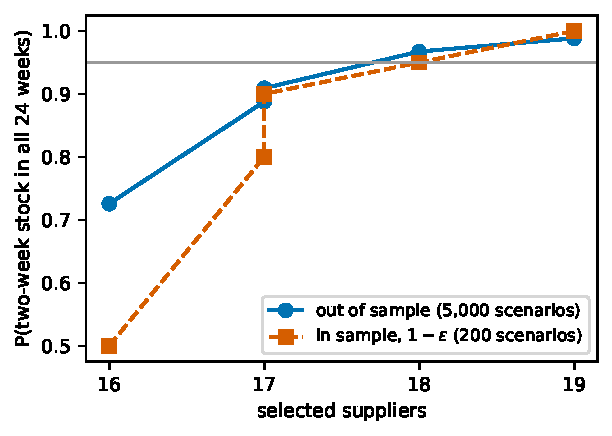
\includegraphics[width=0.58\textwidth]{q2_selection}
\caption{Out-of-sample compliance of the SAA selections compared with their in-sample guarantee $1-\varepsilon$; the grey line is the 95\% target.}\label{fig:sel}
\end{figure}

\subsection{Stability of the Selection}
A selection computed from one sample of 200 scenarios could depend on that sample.
To measure this, we repeated the SAA with $\varepsilon=0.05$ for five independent samples of $N=100$ and $N=200$ scenarios and three samples of $N=400$, and evaluated each selection on 5{,}000 fresh scenarios (\cref{tab:saa-stab}).
Twelve of the thirteen programmes again select 18 suppliers and one selects 17; every selection shares at least 15 suppliers with ours, and one of the $N=400$ samples reproduces it exactly.
The out-of-sample compliance of the 18-supplier sets lies between 93.9\% and 97.0\%, so that the size of the minimum set is stable, while its composition varies at the margin between suppliers of similar score.
Two of the twelve 18-supplier sets fall slightly below 95\%, which confirms that the out-of-sample check is needed and that our selection, at 96.7\%, is one of the more reliable 18-supplier sets.

\begin{table}[ht]
\centering
\caption{Repeated SAA selections with $\varepsilon=0.05$ for independent scenario samples; overlap counts the suppliers shared with the selection of \cref{tab:sel}.}\label{tab:saa-stab}
\small
\begin{tabular}{rrlll}
\toprule
$N$ & samples & suppliers selected & overlap with our set & out-of-sample compliance \\
\midrule
100 & 5 & 18, 17, 18, 18, 18 & 16, 17, 16, 17, 16 & 0.954, 0.910, 0.957, 0.970, 0.962 \\
200 & 5 & 18, 18, 18, 18, 18 & 16, 17, 16, 17, 15 & 0.950, 0.957, 0.966, 0.964, 0.939 \\
400 & 3 & 18, 18, 18 & 18, 17, 17 & 0.968, 0.962, 0.944 \\
\bottomrule
\end{tabular}
\end{table}

A simple heuristic gives an independent check of the size of the minimum set.
Taking the suppliers in the order of $Q_i$ and ordering them at capacity, the 17 highest-ranked suppliers reach a compliance of 91.1\% and the 18 highest-ranked 95.7\%, so the heuristic also needs 18 suppliers.
The SAA set of the same size is more reliable (96.7\%) because it replaces S201, which ranks seventh by score but has a mean ratio of only 0.54, by the more reliable S268 at rank 19.
Both methods thus agree that 18 is the smallest number of suppliers with which the firm can meet the stock requirement with 95\% probability, and the chance-constrained model in addition finds the most reliable composition.

\subsection{Order Plan with an Uncertainty-Dependent Safety Stock}
Ordering all 18 suppliers at capacity in every week is compliant in 96.7\% of the scenarios, but it accumulates far more stock than required: the median stock at the end of the horizon is 4.7 weeks of demand, and the plan costs 541{,}890 (price of C $=1$) over 24 weeks.
The cheapest plan reduces orders where the stock allows it, while protecting against the uncertainty of the deliveries.
Using \cref{eq:moments}, we require the expected cumulative supply to exceed the cumulative demand by a safety stock proportional to its standard deviation, and minimise the expected purchase cost:
\begin{equation}\label{eq:order}
\begin{aligned}
\min_{x}\ & \sum_{i,t}(p_i+w)\,\bar\rho_i\,x_{it}\\
\text{s.t.}\ & \sum_{\tau\le t}\sum_i \frac{\bar\rho_i\,x_{i\tau}}{\alpha_i}\ \ge\ tD + z\,\sigma_t(x), && t=1,\dots,24,\\
& \sum_i \bar\rho_i\,x_{it}\ \le\ 8\times 6{,}000, && t=1,\dots,24,\\
& 0\le x_{it}\le K_i .
\end{aligned}
\end{equation}
The objective counts expected deliveries, because the firm pays for what it receives; the second constraint keeps the expected weekly deliveries within the total carrier capacity; and the parameter $w$, a cost per cubic metre of raw volume, is zero here and used in Problem 3.
The safety term $z\,\sigma_t(x)$ is the classical safety stock of inventory theory \citep{silver2016}, with the difference that it is computed from the variance of the supply, accumulated over the weeks up to $t$, rather than from the variance of demand.

Because $\sigma_t(x)$ depends on the plan itself, \cref{eq:order} is not linear.
We solve it by a fixed-point iteration: starting from $x=K$, we evaluate $\sigma_t$ at the current plan, solve the resulting linear programme, and repeat three times, after which the plan no longer changes noticeably.
The safety factor $z$ is then calibrated by simulation, because the ratio distributions are far from normal and the usual normal quantile would be misleading.
We increase $z$ from zero in steps of 0.25 and accept the first plan that is compliant in 95\% of 2{,}000 fresh scenarios; if \cref{eq:order} becomes infeasible before that, because the capacities of the 18 suppliers cannot provide a larger safety stock, we keep the plan with the largest feasible $z$.

\subsection{Order Plan Results}
For the 18 suppliers, \cref{eq:order} is feasible up to $z=2$, which gives the cheapest plan.
It costs 497{,}856, 8.1\% less than ordering at capacity, is compliant in 91.6\% of the fresh scenarios, never runs out of stock in any scenario, and ends with a median stock of 2.5 weeks (\cref{fig:stock}).
Its cost per unit of product, 0.7204, is practically the same as the historical 0.7221, so the plan reaches the required stock without paying more per unit than the firm did in the past.
The plan expects 154{,}251\,m$^3$ of A, 33{,}579\,m$^3$ of B and 275{,}817\,m$^3$ of C over the 24 weeks; the complete plan is in \texttt{results/q2\_order\_plan.csv}.

The plan has a simple structure that explains its cost.
Fourteen of the 18 suppliers are ordered at their capacity in every week, and only the four suppliers of B, S108, S131, S308 and S340, are used flexibly.
This is exactly what the cost per unit of product predicts: B costs 0.726 per unit of product against 0.720 for A and C (\cref{sec:q3}), so B is the material to cut first.
The 14 suppliers of A and C supply an expected 26{,}674\,m$^3$ of product per week, 5\% less than the demand, so the B suppliers are needed in some weeks; the plan orders all of them at capacity in the first five weeks, building a buffer while the safety requirement is still small, and again in four later weeks, uses some of them partly in five further weeks, and does without them in the remaining ten weeks.
The expected product supplied therefore varies between 26{,}674 and 31{,}321\,m$^3$ per week, with an average of 28{,}793\,m$^3$, 2\% above the demand.
Because the cost depends only on the total quantity ordered from each supplier, the timing of the B orders is not unique; any timing that satisfies the cumulative constraints of \cref{eq:order} costs the same.

\begin{figure}[ht]
\centering
\begin{minipage}[t]{0.48\textwidth}
\centering
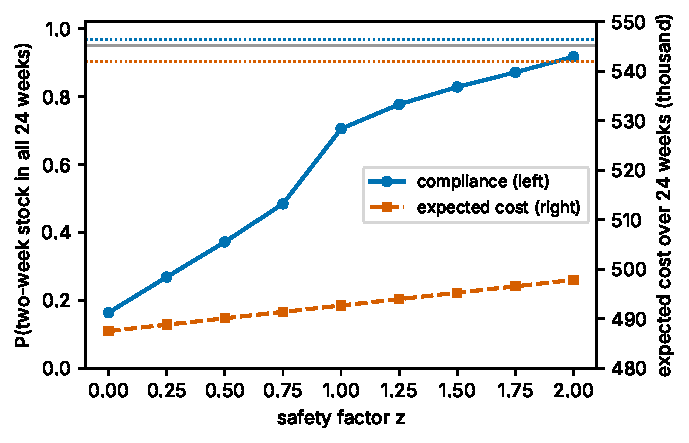
\includegraphics[width=\textwidth]{q2_tradeoff}
\caption{Compliance (left axis) and expected purchase cost (right axis) of the order plans for the 18 suppliers against the safety factor $z$; dotted lines mark ordering every supplier at capacity, the grey line the 95\% target.}\label{fig:tradeoff}
\end{minipage}\hfill
\begin{minipage}[t]{0.48\textwidth}
\centering
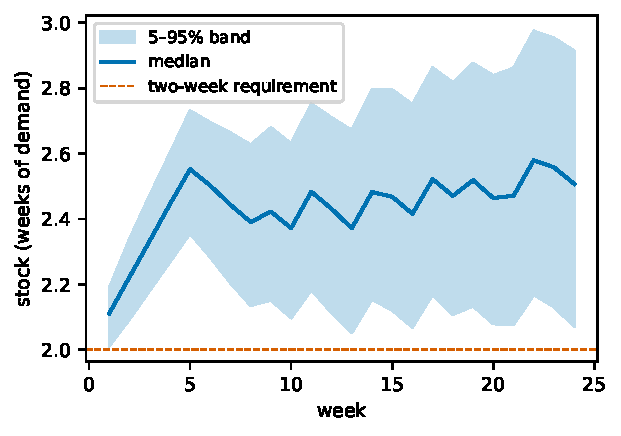
\includegraphics[width=\textwidth]{q2_stock}
\caption{Simulated stock of the cheapest plan ($z=2$, 2{,}000 scenarios): median and 5--95\% band in weeks of demand.}\label{fig:stock}
\end{minipage}
\end{figure}

\Cref{fig:tradeoff} shows how compliance is bought.
Without a safety stock ($z=0$), the plan just keeps the expected stock at two weeks of demand and costs 487{,}516, but it is compliant in only 16.4\% of the scenarios, since in a typical scenario some week falls slightly below the requirement.
Each step of $z$ adds about 1{,}300 to the cost, and compliance rises steeply, to 70.5\% at $z=1$ and 91.7\% at $z=2$, so that the first 75 percentage points of compliance cost only 2.1\% more than the plan without protection.
The last five percentage points are much more expensive: they can only be reached by ordering every supplier at capacity, which costs another 8.8\% and leaves a large surplus stock.
The violations that remain in the cheapest plan are also shallow.
In none of the scenarios does the stock fall below one week of demand, and in 95\% of the scenarios the stock never falls below 1.97 weeks of demand, so a failure of the cheapest plan means a brief and small dip below the two-week buffer rather than a threat to production.
The firm can therefore choose between the cheapest plan with 91.6\% compliance, which we recommend when brief and small violations of the buffer are acceptable, and ordering at capacity for 96.7\% at 8.8\% higher cost.

\subsection{Transport Model}
Given the expected deliveries $d_i=\bar\rho_i x_{it}$ of a week, the transport plan assigns them to carriers so as to minimise the expected loss, subject to the carrier capacities and the rule that a supplier should use one carrier whenever possible.
With continuous volumes $f_{ik}$ and binary indicators $u_{ik}$ for the used supplier--carrier pairs, the weekly model is
\begin{equation}\label{eq:transport}
\begin{aligned}
\min\ & \sum_{i,k}\ell_k f_{ik} + \lambda\sum_{i,k}u_{ik}\\
\text{s.t.}\ & \sum_k f_{ik}=d_i, \qquad \sum_i f_{ik}\le 6{,}000, \qquad 0\le f_{ik}\le\min(d_i,6{,}000)\,u_{ik}, \qquad u_{ik}\in\{0,1\}.
\end{aligned}
\end{equation}
The small penalty $\lambda=0.1$\,m$^3$ per used pair is far below the loss caused by moving one cubic metre to a worse carrier, so it does not change the total loss, but among plans with the same loss it selects the one with the fewest split shipments.
Without the single-carrier rule the problem would be a transportation problem whose solution fills the carriers in the order of increasing loss rate; the binary variables only decide which suppliers fill the remaining capacity of each carrier.
We solve \cref{eq:transport} for each of the 24 weeks with HiGHS, replay the resulting schedule against the actual weekly loss rates of 500 randomly chosen historical 24-week windows (assumption A4), and compare it with random feasible assignments that send each shipment to a random carrier with spare capacity.

\subsection{Transport Results}
The optimal schedule follows the order of the loss rates in \cref{tab:carriers}.
It ships almost all volume through the three carriers with the lowest mean losses, T3 (0.19\%), T6 (0.54\%) and T2 (0.92\%), about 144{,}000\,m$^3$ each over 24 weeks, and the remaining 32{,}826\,m$^3$ through T8 (1.01\%).
In every week the expected deliveries amount to between 17{,}920 and 20{,}987\,m$^3$, so three carriers almost suffice: T3 is filled to its capacity in 22 of the 24 weeks, T6 and T2 carry on average 5{,}993 and 5{,}958\,m$^3$ per week, and T8 takes the remainder in the weeks with the largest orders.
The four carriers with the highest losses are never used.
Only 4 of the 383 supplier-weeks require a second carrier, because every expected delivery, including the largest one of S374 with 4{,}455\,m$^3$, is smaller than the capacity of a carrier, and a split is only worthwhile when the remaining room on a low-loss carrier is too small for a whole delivery.
The expected loss is 2{,}699\,m$^3$, or 0.58\% of the transported volume.
Replayed against the historical weekly loss rates, the schedule loses 0.59\% on average and 0.76\% in the worst 5\% of the windows, against 1.38\% for random feasible assignments.
The optimisation therefore saves about 0.8 percentage points of the transported volume, or roughly 3{,}700\,m$^3$ of raw material over half a year, and its advantage persists when the loss rates fluctuate as they did in the past.
The schedule is given in \texttt{results/q2\_transport\_plan.csv}.

%% ================================================================== 7
\section{Model III: Preference for Material A (Problem 3)}\label{sec:q3}

\subsection{Analysis}
Problem 3 asks to buy as much A and as little C as possible in order to save transport and storage costs.
The reason becomes clear when the three materials are compared per unit of product rather than per cubic metre of raw material.
One cubic metre of product needs $0.60\times1.2=0.720$ units of purchase cost in A, $0.66\times1.1=0.726$ in B and $0.72\times1.0=0.720$ in C, so the purchase cost per unit of product is practically the same for all three materials, with B slightly more expensive.
The raw volume per unit of product, by contrast, is 0.60, 0.66 and 0.72\,m$^3$, so C needs 20\% more volume than A for the same production.
Since transport and storage costs and transport losses all scale with raw volume, preferring A and avoiding C is equivalent to minimising the raw volume of the plan, and this equivalence turns a vague preference into a precise objective.

\subsection{Model}
Volume and cost are two objectives, so we treat them lexicographically and then trace the trade-off between them \citep{ehrgott2005}.
In the first stage we solve \cref{eq:order} over all suppliers with a large weight $w=10$ on raw volume, calibrating the safety factor as in Problem 2, and obtain the minimum expected raw volume $V^*$ of a compliant plan.
In the second stage we minimise the purchase cost subject to the additional constraint that the expected raw volume does not exceed $(1+\delta)V^*$, for $\delta\in\{0,0.5,1,2,5\}\%$ and without a volume limit, keeping the safety stock of the first stage.
This $\varepsilon$-constraint approach shows how much purchase cost each per cent of additional volume saves, and the transport model \cref{eq:transport} is then applied to the plans at both ends of the trade-off.
We use all suppliers rather than the 18 of Problem 2, because the minimum set does not contain enough capacity of A to express the preference.

\subsection{Results}
The volume-minimal plan (\cref{tab:q3}, \cref{fig:mix}) buys all 229{,}248\,m$^3$ of A that the sustained capacities allow over 24 weeks, 108{,}901\,m$^3$ of B and 107{,}159\,m$^3$ of C, a total of $V^*=445{,}307$\,m$^3$, and is compliant in 96.8\% of the scenarios with $z=2.25$.
The cheapest plan without a volume limit uses less A (186{,}244\,m$^3$), no B at all and 2.6 times as much C (277{,}565\,m$^3$); it needs 4.2\% more volume and saves only 0.2\% of the purchase cost (501{,}057 against 502{,}047).
Between the two extremes the mix changes in a characteristic order.
As the volume slack grows, the plan first replaces B by C, because B is the most expensive material per unit of product, while A stays at its maximum; at 2\% of slack C has already risen to 214{,}033\,m$^3$ and B has almost disappeared, and only beyond that does C start to replace A as well.

The trade-off is extremely flat: the whole range from the volume-minimal to the cost-minimal plan spans 0.2\% of the purchase cost but 4.2\% of the volume.
Since transport and storage costs are proportional to volume, the volume-minimal plan is cheaper overall as soon as they exceed $990/18{,}501\approx0.054$ per cubic metre, about 5\% of the average purchase price of a cubic metre, which is a modest share for bulk materials.
The volume-minimal plan also lowers the transport loss rate from 0.64\% to 0.61\%: the carriers with the lowest losses are filled first in either case, so a smaller total volume leaves a smaller share for the worse carriers.
Note that both plans use many more suppliers than Problem 2 (225 and 153), since the preference for A requires the capacity of many small A suppliers; Problem 3 does not ask for a small supplier set, and a firm that wants both would add a cardinality constraint.
We therefore recommend the volume-minimal plan, which cuts the volume of C by 61\% and the total volume by 4.0\% for a 0.2\% higher purchase cost.

\begin{table}[ht]
\centering
\caption{Volume--cost trade-off over all suppliers: expected raw volume (m$^3$ over 24 weeks), purchase cost and compliance on 1{,}000 fresh scenarios.}\label{tab:q3}
\small
\begin{tabular}{lrrrrrr}
\toprule
volume slack $\delta$ & A & B & C & total & cost & compliance \\
\midrule
0 & 229{,}248 & 108{,}901 & 107{,}159 & 445{,}307 & 502{,}047 & 0.968 \\
0.5\% & 229{,}248 & 84{,}409 & 133{,}877 & 447{,}534 & 501{,}824 & 0.972 \\
1\% & 229{,}248 & 59{,}917 & 160{,}596 & 449{,}761 & 501{,}602 & 0.972 \\
2\% & 229{,}248 & 10{,}933 & 214{,}033 & 454{,}214 & 501{,}156 & 0.941 \\
5\% & 181{,}488 & 0 & 283{,}271 & 464{,}759 & 501{,}057 & 0.970 \\
none & 186{,}244 & 0 & 277{,}565 & 463{,}808 & 501{,}057 & 0.972 \\
\bottomrule
\end{tabular}
\end{table}

\begin{figure}[ht]
\centering
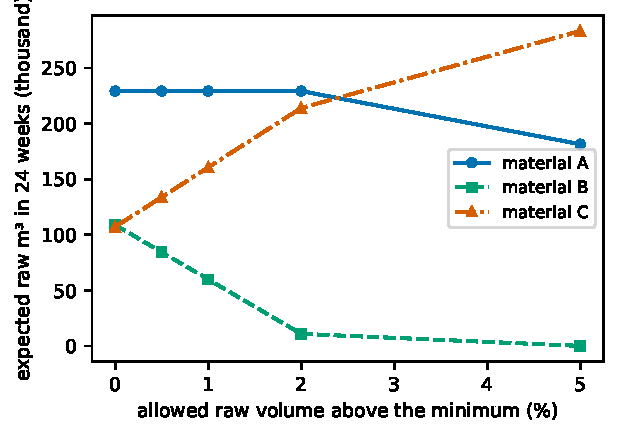
\includegraphics[width=0.58\textwidth]{q3_mix}
\caption{Expected 24-week volume of each material as the allowed raw volume above the minimum grows.}\label{fig:mix}
\end{figure}

The 5\% row of \cref{tab:q3} costs the same as the unconstrained plan but uses slightly more volume, because once the volume constraint is no longer binding the linear programme is indifferent between plans of equal cost and returns a different vertex.
The compliance of all plans lies between 94\% and 97\%, so the volume preference is obtained without loss of reliability; the value 0.941 at 2\% slack lies only 1.3 standard errors of a 1{,}000-scenario estimate below the target.

%% ================================================================== 8
\section{Model IV: Capacity Expansion (Problem 4)}\label{sec:q4}

\subsection{Model}
Problem 4 asks how far weekly production can be raised with the existing suppliers and carriers.
We call a production level $P$ sustainable if the order model \cref{eq:order}, with $D$ replaced by $P$, all suppliers available and the safety factor calibrated as before, yields a plan that is compliant in at least 95\% of 500 fresh scenarios.
A higher production raises both the required stock and the weekly consumption, so the compliance of the best plan decreases with $P$, and the largest sustainable level can be found by bisection between $P=0.5D$ and the total expected capacity.
Twelve bisection steps narrow the interval to less than 0.03\% of its initial width.
Because the answer rests directly on the capacities, we compute it for every window $W$ and also record the peak weekly transport volume to see whether the carriers become a bottleneck.

\subsection{Results}
With the base capacity ($W=4$), the largest sustainable production is 37{,}749\,m$^3$ per week, 34\% above the current 28{,}200\,m$^3$ (\cref{tab:q4}).
At this level the plan's peak weekly transport volume is 28{,}403\,m$^3$, well below the 48{,}000\,m$^3$ that the eight carriers can move, so production is limited by the suppliers and not by transport.
The expected capacity of all suppliers is 42{,}675\,m$^3$ per week, so about 88\% of it can be turned into reliable production; the remaining 12\% is needed as protection against the variability of the deliveries.

\Cref{fig:q4} shows how compliance changes with production when the plan is re-optimised for each level.
Up to about 37{,}000\,m$^3$ per week, the calibrated plans keep compliance between 95\% and 97\%, because the safety factor can be raised as production grows; beyond this point the suppliers have no spare capacity left for a safety stock, and compliance falls steeply, to 92\% at 38{,}000, 73\% at 40{,}000 and 29\% at 42{,}000\,m$^3$ per week.
This cliff has a useful consequence: the production limit hardly depends on the required service level.
Repeating the bisection with targets of 90\%, 95\% and 99\% gives 38{,}461, 37{,}868 and 36{,}849\,m$^3$ per week, increases of 36\%, 34\% and 31\%.
The second value differs from that of \cref{tab:q4} by 0.3\% because it uses fresh scenarios, which gives an idea of the simulation error.
We therefore report the production limit as about 37{,}700\,m$^3$ per week, or an increase of roughly one third.

\begin{figure}[ht]
\centering
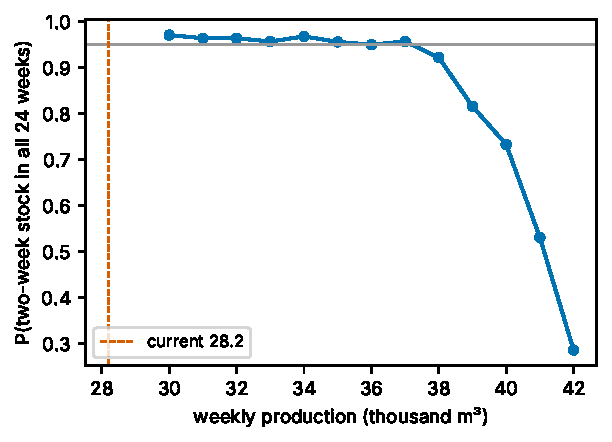
\includegraphics[width=0.58\textwidth]{q4_curve}
\caption{Compliance of the re-optimised plan over all suppliers as a function of weekly production ($W=4$; 1{,}000 fresh scenarios per point).}\label{fig:q4}
\end{figure}

\begin{table}[ht]
\centering
\caption{Maximum production sustainable with 95\% compliance (500 fresh scenarios per bisection step) for different capacity windows.}\label{tab:q4}
\small
\begin{tabular}{rrrrr}
\toprule
window $W$ & expected capacity & max production & change & peak transport (m$^3$/week) \\
\midrule
3 & 81{,}778 & 56{,}564 & +101\% & 48{,}000 \\
4 & 42{,}675 & 37{,}749 & +34\% & 28{,}403 \\
6 & 31{,}156 & 27{,}816 & $-1\%$ & 20{,}449 \\
8 & 28{,}011 & 25{,}158 & $-11\%$ & 18{,}409 \\
\bottomrule
\end{tabular}
\end{table}

%% ================================================================== 9
\section{Model Testing and Sensitivity Analysis}\label{sec:sensitivity}

\subsection{Out-of-Sample Testing}
Every selection and every order plan in this paper is evaluated on scenarios that were not used to construct it: 5{,}000 for the selections, 2{,}000 for the order plans of Problem 2, 1{,}000 in Problem 3 and 500 per bisection step in Problem 4.
This test reveals two kinds of optimism that would otherwise go unnoticed.
The deterministic answer of 15 suppliers, which is feasible on average, keeps the stock in only 40\% of the scenarios.
The SAA guarantee is not reliable either: at $\varepsilon=0.05$ the 18 suppliers exceed their guarantee (96.7\% against 95\%), but at $\varepsilon=0.1$ the true compliance (90.9\%) is barely at the guarantee, and two of the repeated samples of \cref{tab:saa-stab} fall below their guarantee of 95\%.
Selecting $\varepsilon$ by out-of-sample compliance instead of setting it to the target removes this optimism at the cost of solving a few more programmes.

\subsection{Correlated Deliveries}\label{sec:sens-corr}
Assumption A2 treats the delivery ratios as independent across suppliers and weeks.
If suppliers tend to fail together, for example because of weather or a common transport disruption, or if a bad week tends to be followed by another, the true compliance would be lower.
We test this assumption in two ways.
First, we measure the dependence in the records: over the weeks in which both were ordered, the delivery ratios of pairs of the 18 selected suppliers have a median correlation of $-0.01$, and 90\% of the pairs have a correlation below 0.09; the median lag-one autocorrelation of a supplier's ratios is $-0.02$.
Second, we replace the independent resampling by a block bootstrap of historical weeks: each scenario consists of six blocks of four consecutive historical weeks, and all suppliers take the ratios of the same weeks, so that any common shocks and short-run persistence in the records are carried into the scenarios.
Where a supplier was not ordered in a sampled week, its ratio is drawn from its own history as before.

\begin{table}[ht]
\centering
\caption{Compliance of the 18-supplier plans under independent resampling and under a bootstrap of common historical weeks (5{,}000 scenarios each).}\label{tab:stress}
\small
\begin{tabular}{lrrr}
\toprule
Plan & independent & common weeks & common 4-week blocks \\
\midrule
all 18 at capacity & 0.972 & 0.972 & 0.969 \\
cheapest plan ($z=2$) & 0.911 & 0.920 & 0.894 \\
\bottomrule
\end{tabular}
\end{table}

\Cref{tab:stress} shows that the selection is robust to the dependence present in the records: ordered at capacity, the 18 suppliers keep a compliance of about 97\% under all three schemes.
The cheapest plan, whose safety stock is thinner, loses 1.7 percentage points under four-week blocks, which is the largest effect of correlation we found.
The independence assumption is therefore adequate for the 240 recorded weeks, although a disruption that affects many suppliers at once and is absent from the records would not be captured by either scheme.

\subsection{Capacity Definition}\label{sec:sens-window}
The window $W$ in \cref{eq:K} is the least certain modelling choice, and its influence differs strongly between the problems.
For Problem 1 the top 50 change by at most two suppliers across $W=3,6,8$ (\cref{tab:q1rob}).
For Problem 4, by contrast, the window dominates the answer (\cref{tab:q4}).
With $W=3$ production could double, but the carriers would then be fully used in the peak week (48{,}000\,m$^3$), so transport becomes the bottleneck and the answer rests on short bursts of a few suppliers that may not be repeatable.
With $W=6$ or $8$ even the current production is not sustainable at 95\%. The value for $W=6$, 27{,}816\,m$^3$, is close to the 27{,}933\,m$^3$ that the firm actually received per week on average, which indicates that long windows mainly reproduce the historical deliveries, which were limited by the orders, rather than the capacities.
The base case $W=4$ lies between these extremes and is the shortest window that excludes isolated spikes of one or two weeks.
The production estimate of Problem 4 should therefore be read together with the capacity definition it rests on, and a firm that wants to rely on it should confirm the capacities of its largest suppliers directly.

\subsection{Ratio Cap, Demand and Capacity Errors}\label{sec:sens-param}
\Cref{tab:sens} varies three further inputs one at a time and records the compliance of the 18 suppliers ordered at capacity.
The cap on the delivery ratio matters little: lowering it from 1.5 to 1.2 reduces compliance from 97.0\% to 96.2\%, and removing it changes nothing, because large ratios occur mostly for small orders.
Demand and capacity matter much more.
A demand that is 2\% higher than planned lowers compliance to 93.8\%, and 5\% to 85.4\%; capacities that are 5\% lower than estimated lower it to 84.6\%.
This sensitivity is the other side of a minimum supplier set: the expected supply of the 18 suppliers exceeds the demand by only 11\%, and most of this margin is needed as protection against random deliveries.
A firm that expects demand growth or doubts the capacity estimates should therefore add a nineteenth supplier, which by \cref{tab:sel} raises compliance to 98.8\%.

\begin{table}[ht]
\centering
\caption{Sensitivity of the compliance of the 18 suppliers ordered at capacity (5{,}000 scenarios each). The base value 0.970 differs from the 0.967 of \cref{tab:sel} only by sampling error.}\label{tab:sens}
\small
\begin{tabular}{lrrrr}
\toprule
Ratio cap & 1.2 & 1.5 (base) & 2.0 & none \\
compliance & 0.962 & 0.970 & 0.972 & 0.971 \\
\midrule
Demand factor & 0.95 & 0.98 & 1.02 & 1.05 \\
compliance & 0.997 & 0.990 & 0.938 & 0.854 \\
\midrule
Capacity factor & 0.95 & & & 1.05 \\
compliance & 0.846 & & & 0.998 \\
\bottomrule
\end{tabular}
\end{table}

\subsection{Transport Loss Rates}
The transport plans are computed with mean loss rates, while the actual rates fluctuate from week to week.
Replaying the schedule of Problem 2 against 500 historical 24-week windows gives a mean loss rate of 0.59\% and a 95th percentile of 0.76\%, close to the planned 0.58\%.
Although single weeks can be much worse than the mean (\cref{tab:carriers}), the fluctuations largely average out over the 24 weeks and over the three carriers that carry most of the volume, so the plan computed from mean rates remains close to the best achievable.

%% ================================================================== 10
\section{Model Evaluation and Extension}\label{sec:evaluation}

\subsection{Strengths}
The main strength of the approach is that it separates what the data identify, the distribution of the delivery ratios, from what they do not identify, the capacities, and that it makes the capacity assumption explicit in a single parameter whose influence can be measured.
The importance score of Problem 1 follows from the stock balance rather than from an arbitrary weighting, and it agrees with an independent multi-criteria evaluation.
The selection of Problem 2 is computed by an exact chance-constrained programme and remains stable across scenario samples, and every decision is checked on scenarios not used for optimisation, which guards against both the optimism of expected values and that of small-sample guarantees.
All programmes are solved to optimality by an open-source solver within minutes, so the plans can be recomputed every week as new deliveries are recorded.

\subsection{Weaknesses}
The supply model also limits the conclusions.
The delivery ratios are resampled independently, and although the stress test of \cref{sec:sens-corr} found little correlation in the records, a disruption that affects many suppliers at once, which the 240 weeks may not contain, would lower the compliance.
Orders up to the sustained capacity are assumed to be delivered with the historical ratio distribution, which cannot be checked for suppliers that were never ordered this much.
The sustained capacity uses one window for all suppliers, and Problem 4 shows that this choice dominates the production limit.
Finally, the transport model uses expected deliveries, and the plans of Problems 3 and 4 do not limit the number of suppliers.

\subsection{Extensions}
Three extensions would address these weaknesses.
A two-stage or rolling-horizon stochastic programme, in which orders are revised each week after the deliveries of the previous week are observed, would let the firm react to shortfalls and would lower the cost of compliance compared with the static plan.
A censored-demand (Tobit-type) model of deliveries, which treats a delivery as the minimum of the order and an unobserved capacity, could estimate a capacity distribution for each supplier and season instead of a single window.
A cardinality constraint in Problems 3 and 4 would show how much of the volume saving and the production increase can be obtained with a small supplier base.

%% ================================================================== 11
\section{Conclusions}
Ranked by the product they can reliably supply, the 50 most important suppliers hold 98.8\% of the sustained capacity, and this ranking is robust both to the capacity definition and to the evaluation method.
Production can be sustained with as few as 18 suppliers at 96.7\% compliance, three more than an analysis of expected values suggests; for them the cheapest order plan reaches 91.6\% compliance at the historical cost per unit of product, and the optimised transport plan loses 0.58\% of the material, less than half of a random assignment.
Because the three materials cost almost the same per unit of product, a preference for A is a preference for low volume, and the volume-minimal plan cuts C by 61\% and the total volume by 4.0\% for a 0.2\% higher purchase cost.
With the existing suppliers and carriers, weekly production can rise to about 37{,}700\,m$^3$ (+34\%) under the base capacity definition, limited by the suppliers rather than by the carriers, although this estimate ranges from $-11\%$ to $+101\%$ across capacity definitions.
The common lesson of the four problems is that the variability of the deliveries, rather than their mean, determines how many suppliers are needed and how much can be produced, and that it should be measured on scenarios independent of the plan.

\begingroup
\small
\begin{thebibliography}{99}
\bibitem[Aissaoui et~al.(2007)]{aissaoui2007} N.~Aissaoui, M.~Haouari, and E.~Hassini. Supplier selection and order lot sizing modeling: A review. \emph{Computers \& Operations Research}, 34(12):3516--3540, 2007.
\bibitem[Charnes and Cooper(1959)]{charnes1959} A.~Charnes and W.~W. Cooper. Chance-constrained programming. \emph{Management Science}, 6(1):73--79, 1959.
\bibitem[Ehrgott(2005)]{ehrgott2005} M.~Ehrgott. \emph{Multicriteria Optimization}. Springer, Berlin, 2nd edition, 2005.
\bibitem[Ho et~al.(2010)]{ho2010} W.~Ho, X.~Xu, and P.~K. Dey. Multi-criteria decision making approaches for supplier evaluation and selection: A literature review. \emph{European Journal of Operational Research}, 202(1):16--24, 2010.
\bibitem[Huangfu and Hall(2018)]{huangfu2018} Q.~Huangfu and J.~A.~J. Hall. Parallelizing the dual revised simplex method. \emph{Mathematical Programming Computation}, 10(1):119--142, 2018.
\bibitem[Hwang and Yoon(1981)]{hwang1981} C.-L. Hwang and K.~Yoon. \emph{Multiple Attribute Decision Making: Methods and Applications}. Springer, Berlin, 1981.
\bibitem[Luedtke and Ahmed(2008)]{luedtke2008} J.~Luedtke and S.~Ahmed. A sample approximation approach for optimization with probabilistic constraints. \emph{SIAM Journal on Optimization}, 19(2):674--699, 2008.
\bibitem[Pagnoncelli et~al.(2009)]{pagnoncelli2009} B.~K. Pagnoncelli, S.~Ahmed, and A.~Shapiro. Sample average approximation method for chance constrained programming: Theory and applications. \emph{Journal of Optimization Theory and Applications}, 142(2):399--416, 2009.
\bibitem[Silver et~al.(2016)]{silver2016} E.~A. Silver, D.~F. Pyke, and D.~J. Thomas. \emph{Inventory and Production Management in Supply Chains}. CRC Press, Boca Raton, 4th edition, 2016.
\end{thebibliography}
\endgroup

\appendix
\section{Programs and Data}
All results are produced by two scripts (Python 3.9, NumPy 2.0.2, SciPy 1.13.1 with HiGHS, fixed seeds).
\texttt{code/run\_all.py} computes the supply model and the main results of the four problems in about 20 minutes, and \texttt{code/supplementary.py} computes the additional analyses of \cref{sec:model,sec:q1,sec:q2,sec:q4,sec:sensitivity} from its outputs.

\begin{center}
\small
\begin{tabular}{lp{0.42\textwidth}}
\toprule
File & Content \\
\midrule
\texttt{data/attachment1\_suppliers.xlsx} & orders and deliveries, 402 suppliers $\times$ 240 weeks \\
\texttt{data/attachment2\_transporters.xlsx} & loss rates, 8 carriers $\times$ 240 weeks \\
\texttt{results/supplier\_model.csv} & capacities and ratio statistics (\cref{sec:model}) \\
\texttt{results/q1\_top50.csv}, \texttt{q1\_robustness.csv} & \cref{tab:top50,tab:q1rob} \\
\texttt{results/q2\_selection.csv} & \cref{tab:sel} \\
\texttt{results/q2\_order\_plan.csv} & order plan of Problem 2 \\
\texttt{results/q2\_transport\_plan.csv} & transport plan of Problem 2 \\
\texttt{results/q3\_lexicographic.csv} & \cref{tab:q3} \\
\texttt{results/q4\_capacity.csv} & \cref{tab:q4} \\
\texttt{results/supplementary/} & \cref{tab:carriers}, TOPSIS ranking, SAA stability, stress test, trade-off, Problem 4 curve, sensitivity \\
\bottomrule
\end{tabular}
\end{center}

\end{document}
